\chapter{Management Summary}
\label{chapter:management_summary} 



Analysen des Penetrations-Test haben ergeben, dass 8 von 10 gefundenen Hosts innerhalb der Netzwerkinfrastruktur von MB-Reps kompromittiert werden konnten und 13 verschiedene Schwachstellen aufgedeckt wurden. Die Schwere der Schwachstellen erlaubt es einem externen und nicht authentifizierten Angreifer das gesamte Firmennetzwerk (abgesehen von der externen und internen Firewall) zu übernehmen. Die Risikoeinscheinschätzung für die Kunden-Netzwerkinfrastruktur wird daher mit \textcolor{red}{HOCH} bewertet. Es wird empfohlen umgehend Maßnahmen zur Absicherung der IT-Infrastruktur einzuleiten. Über den offiziellen Web-Auftritt der Firma MB-Reps konnte initial der Host \texttt{myron} kompromittiert sowie Administrations-Berechtigungen erlangt werden. Aufgrund dessen wird empfohlen, die Erreichbarkeit des Webauftritts schnellstmöglich abzuschalten und die Softwareschwachstelle des web-basierten Ping-Tools zu beheben sowie die Passwörter des Benutzers \texttt{myron} zu ändern und eine 2-Faktor-Authentifizierung für im Internet befindlichen Systeme einzuführen. Generell wird empfohlen eine interne Passwort-Policy in Form eines Workshops zu errichten und alle Mitarbeiter mit dem sicheren Umgang von Passwörtern zu schulen, da unsichere Passwörter mit Wörterbuchangriffen über mehrere Systeme und Konten hinweg gebrochen werden konnten. Neben der Passwort-Policy wird empfohlen, einheitliche Administrations-Konten mit unterschiedlichen Passwörtern auf allen Firmen-Systemen einzurichten und zentral von der IT-Abteilung zu verwalten. Administrations-Konten sollten dabei keinem Standard-Benutzer zugeordnet werden, um die Ausweitung der Rechte und das Berechtigungsmanagmenet zu vereinfachen. Darüber hinaus sollten schnellstmöglich alle Systeme auf den aktuellsten Stand aktualisiert werden, da einige System aufgrund von bekannten Schwachstellen übernommen werden konnten. Neben den Betriebssystem-Updates sollten auch die betriebenen Software-Applikationen aktualisiert werden. Eine strikte Update-Policy zum aktualisieren von bestehenden Systemen sollte im Rahmen eines Workshops ausgearbeitet und etabliert werden. Darüber hinaus konnten Indizien auf einen Innentäter ausgehend vom Benutzer \texttt{Lightman} des Systems \texttt{Esperanza} ausfindig gemacht werden. Daher sollten umgehend interne forensische Ermittlungen, mit einem professionellen Incident-Response-Team, durchgeführt werden.

Tabelle \ref{tab:vuln_systems} listet die kompromittierten Systeme inkl. Angabe der erlangten Berechtigungen auf. Darüber hinaus zeigt Abbildung \ref{fig:vuln_overview} die Angriffsvektoren und die kompromittierten Systeme in Form eines Netzwerkdiagrams auf. 

\begin{table}[h!]
	\centering
	\begin{tabular}[h]{|l|c|}
		\hline
		\textbf{System} & \textbf{Erlangte Berechtigungen} \\
		\hline
		myron (DMZ) & Administrations-Berechtigungen \\
		\hline
		spoon (DMZ) & Administrations-Berechtigungen \\
		\hline
		win (internes Netzwerk)  & Administrations-Berechtigungen \\
		\hline
		BigCindy (internes Netzwerk)  & Administrations-Berechtigungen \\
		\hline
		Esperanza (internes Netzwerk)  & Administrations-Berechtigungen \\
		\hline
		Mickey (internes Netzwerk)  & Administrations-Berechtigungen \\
		\hline
	\end{tabular}
	\caption{Auflistung der kompromittierten Systeme}
	\label{tab:vuln_systems}
\end{table}


\begin{figure}[h]
	\centering
	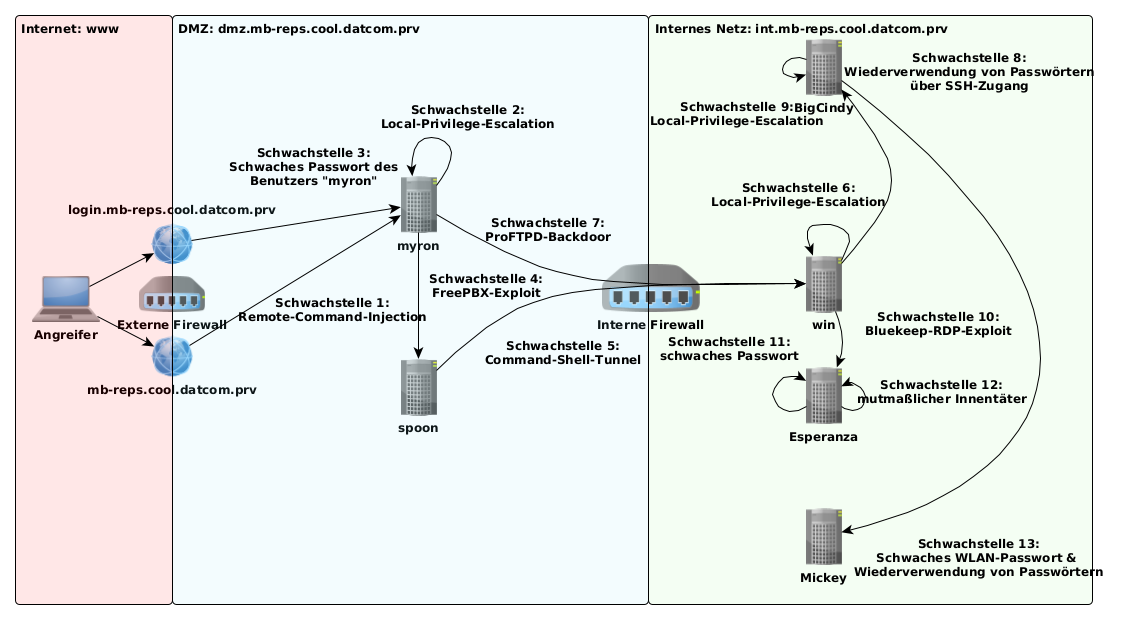
\includegraphics[width=\textwidth]{./img/vuln_overview}
	\caption{Darstellung der Netzwerk-Infrastruktur inkl. aller gefundenen Schwachstellen.}
	\label{fig:vuln_overview}
\end{figure}
